
\section{Results of Modifications}



\begin{frame}
\frametitle{Results of Modifications -- Autoassociative Memory}

\only<1>{
    \begin{figure}
        \centering
        \caption*{\(n=2\)}
        \begin{subfigure}{0.5\textwidth}
            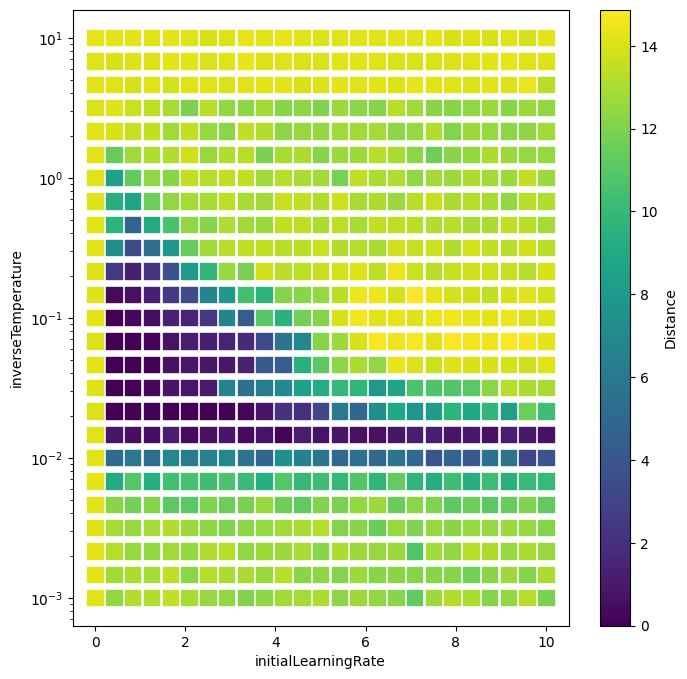
\includegraphics[width=\textwidth]{images/afterHyperparameterSearches/original/Scatter-interactionVertex002.png}
            \caption*{Original}
        \end{subfigure}%
        ~
        \begin{subfigure}{0.5\textwidth}
            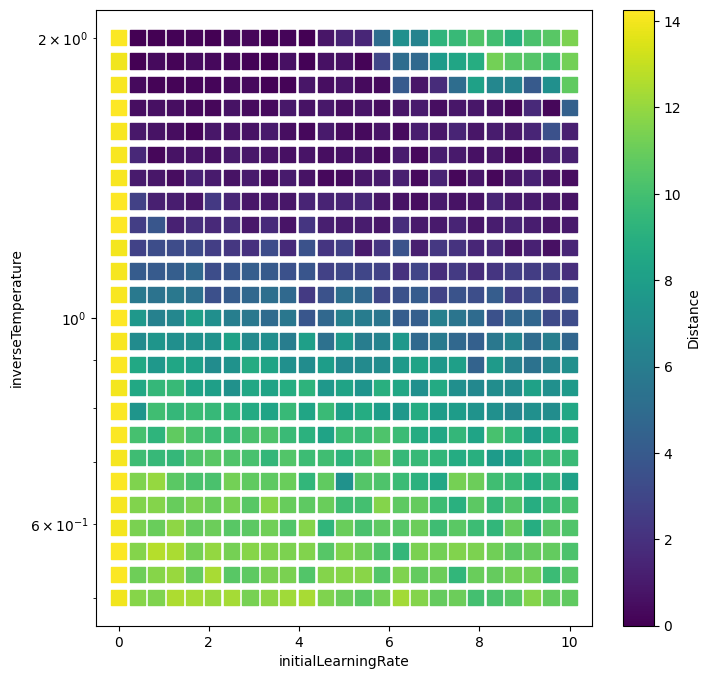
\includegraphics[width=\textwidth]{images/afterHyperparameterSearches/modified/Scatter-interactionVertex002.png}
            \caption*{Modified}
        \end{subfigure}
    \end{figure}
}

\only<2>{
    \begin{figure}
        \centering
        \caption*{\(n=10\)}
        \begin{subfigure}{0.5\textwidth}
            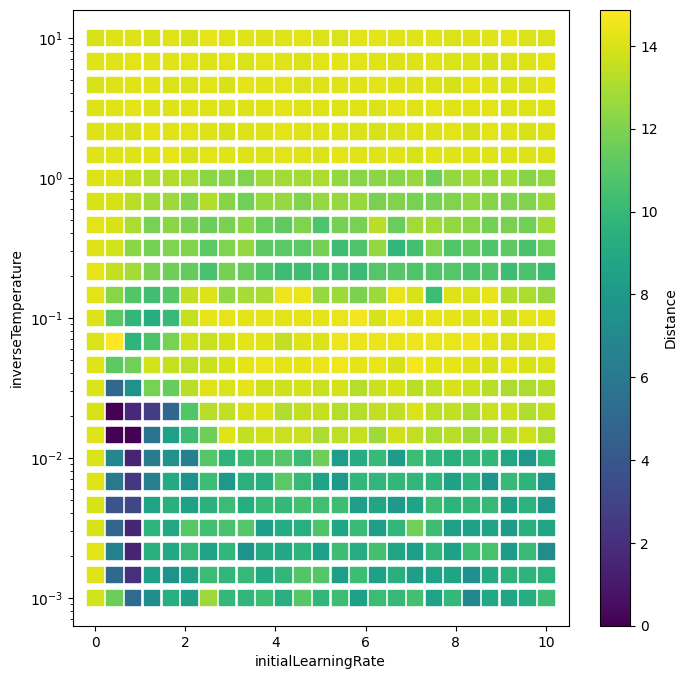
\includegraphics[width=\textwidth]{images/afterHyperparameterSearches/original/Scatter-interactionVertex010.png}
            \caption*{Original}
        \end{subfigure}%
        ~
        \begin{subfigure}{0.5\textwidth}
            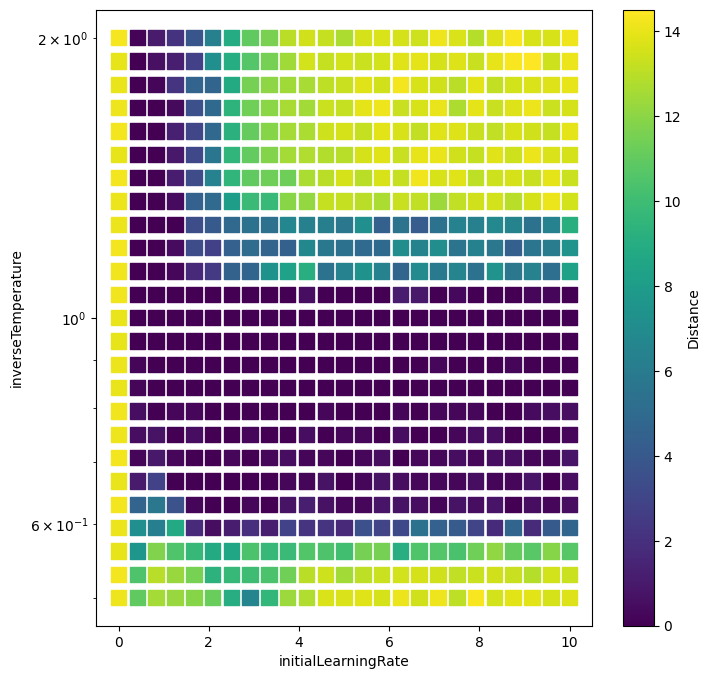
\includegraphics[width=\textwidth]{images/afterHyperparameterSearches/modified/Scatter-interactionVertex010.png}
            \caption*{Modified}
        \end{subfigure}
    \end{figure}
}

\only<3>{
    \begin{figure}
        \centering
        \caption*{\(n=20\)}
        \begin{subfigure}{0.5\textwidth}
            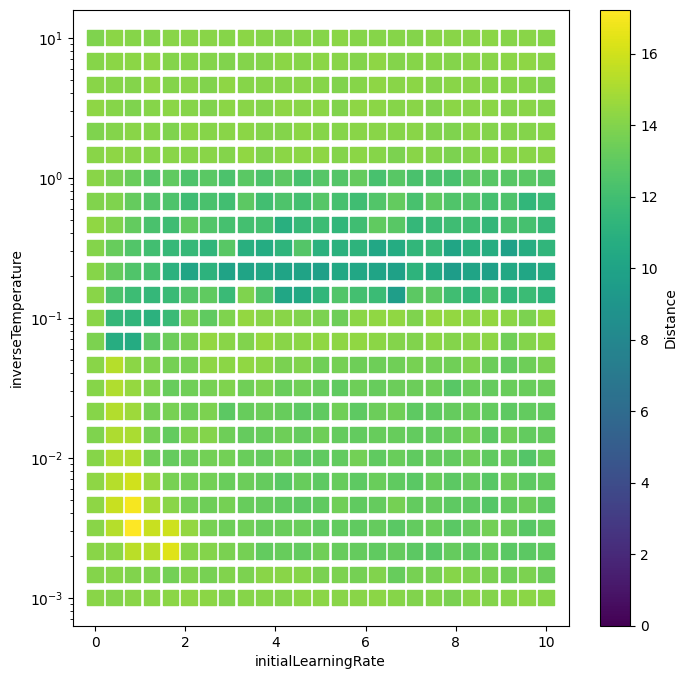
\includegraphics[width=\textwidth]{images/afterHyperparameterSearches/original/Scatter-interactionVertex020.png}
            \caption*{Original}
        \end{subfigure}%
        ~
        \begin{subfigure}{0.5\textwidth}
            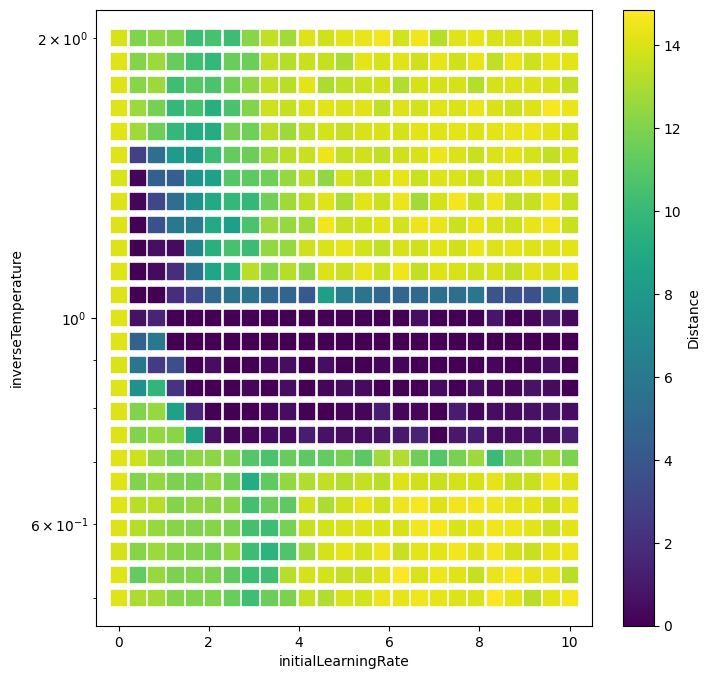
\includegraphics[width=\textwidth]{images/afterHyperparameterSearches/modified/Scatter-interactionVertex020.png}
            \caption*{Modified}
        \end{subfigure}
    \end{figure}
}

\end{frame}

\begin{frame}
    \frametitle{Results of Modifications -- MNIST Classification}

    \only<1>{
        \begin{figure}
            \centering
            \caption*{\(n=2\)}
            \begin{subfigure}{0.5\textwidth}
                % TODO
                % \includegraphics[width=\textwidth]{images/MNISTresults/original 02.png}
                \caption*{Original}
            \end{subfigure}%
            ~
            \begin{subfigure}{0.5\textwidth}
                % TODO
                % \includegraphics[width=\textwidth]{images/MNISTresults/modified 02.png}
                \caption*{Modified}
            \end{subfigure}
        \end{figure}
    }

    \only<2>{
        \begin{figure}
            \centering
            \caption*{\(n=10\)}
            \begin{subfigure}{0.5\textwidth}
                % TODO
                % \includegraphics[width=\textwidth]{images/MNISTresults/original 02.png}
                \caption*{Original}
            \end{subfigure}%
            ~
            \begin{subfigure}{0.5\textwidth}
                % TODO
                % \includegraphics[width=\textwidth]{images/MNISTresults/modified 02.png}
                \caption*{Modified}
            \end{subfigure}
        \end{figure}
    }
    
\end{frame}

\begin{frame}
    \frametitle{Properties -- Feature to Prototype Transition}

Low interaction vertices result in memories that look like features, while higher interaction vertices result in memories that look like prototypes:

\begin{columns}
    \column{.5\textwidth}
    \begin{figure}
        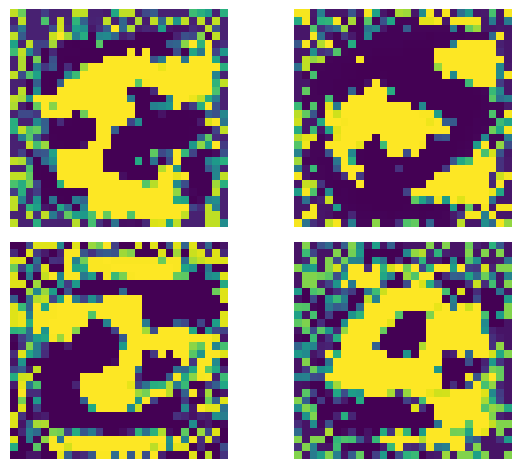
\includegraphics[width=\textwidth]{images/featureDetector.png}
        \caption{Feature-like Memories, \(n=2\)}
    \end{figure}
    \pause
    \column{.5\textwidth}
    \begin{figure}
        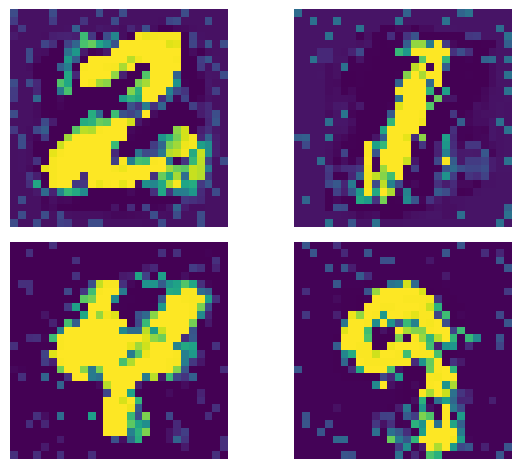
\includegraphics[width=\textwidth]{images/prototypeMemory.png}
        \caption{Prototype-like Memories, \(n=20\)}
    \end{figure}
\end{columns}
\end{frame}